% Format:  Latex Orientation:  Portrait
% MASTERFILE
%
% Last change: <Thu, 2016/05/26 10:25:26 arwagner l00slwagner.desy.de>
%
\documentclass[presentation, 10pt]{beamer}
% use ``handout'' instead of ``presentation'' to create a 2 on 1 page
% handout version of the document

\mode<handout>{%
	\usepackage{pgf}
	\usepackage{pgfpages}
	\pgfpagesuselayout{2 on 1}[a4paper,border shrink=5mm]
}
\mode<presentation>{%
	\usetheme{DESY}
}
%% Setup for Beamer
\usepackage{xcolor}
\usepackage{hyperxmp}
% \usepackage[pdfa]{hyperref}
\usepackage{luatextra}
\usepackage{wasysym}
\usepackage{eurosym}
\usepackage{bookmark}
\usepackage{graphicx}
\usepackage{fontspec}
\setmainfont{Arial}
\usepackage[ngerman,english]{babel}
\usepackage{xspace}
\usepackage{tikz}

\tikzset{%
  every overlay node/.style={%
    %draw=black,fill=white,rounded corners,anchor=north west,
    draw=fzjlightblue,fill=fzjgray30,rounded corners,anchor=north west,
  },
}
% Usage:
% \tikzoverlay at (-1cm,-5cm) {content};
% or
% \tikzoverlay[text width=5cm] at (-1cm,-5cm) {content};
\def\tikzoverlay{%
   \tikz[baseline,overlay]\node[every overlay node]
}%


% General new commands an macros
\renewcommand{\emph}[1]{\structure{#1}}

\newcommand{\link}[2]{\href{#1}{~#2}}

\newcommand{\jointwo}{\textbf{JOIN$^2$}\xspace}

\newcommand{\BibTeX}{Bib\TeX}
\newcommand{\JabRef}{\link{http://jabref.sf.net}{JabRef}\xspace}
\newcommand{\Companion}[1]{\textit{\link{http://julib.fz-juelich.de/uhtbin/field-search-sort/001/PBYR/213964}{\LaTeX{} Companion}, #1}\xspace}
\newcommand{\pkg}[1]{\emph{\texttt{#1}}\xspace}

% general colour definitions
\newcommand{\smallgray}[1]{{\tiny\emph{#1}}}

\newcommand{\idR}{i.~d.~R.\xspace}
\newcommand{\va}{v.~a.\xspace}
\newcommand{\sa}{s.~a.\xspace}
\newcommand{\zB}{z.~B.\xspace}
\newcommand{\zT}{z.~T.\xspace}
\newcommand{\ggf}{ggf.\xspace}
\newcommand{\eg}{e.~g.\xspace}

\newcommand{\bs}[1]{\texttt{$\backslash$#1}}
\newcommand{\command}[2]{\texttt{\bs{#1}\{#2\}}}
% http://tex.stackexchange.com/questions/16447/beamer-top-aligning-columns-within-a-top-aligned-fram
\makeatletter
\newenvironment{topitemize}{%
   \setlength{\topsep}{0pt}
   \setlength{\partopsep}{0pt}
   \renewcommand*{\@listi}{\leftmargin\leftmargini \parsep\z@ \topsep\z@ \itemsep\z@}
   \let\@listI\@listi
   \itemize
}{\enditemize}
\makeatother


\title{The DQM4hep project}
% subtitle is required for DESY beamer, set at least a space ~
\subtitle{CHEP 2018 conference}

\author[R. Ete]{\underline{R\'emi Ete}, Antoine Pingault}
\institute{DESY}
\date{July 10, 2018}

\newenvironment{topitemize}{%
   \setlength{\topsep}{0pt}
   \setlength{\partopsep}{0pt}
   \renewcommand*{\@listi}{\leftmargin\leftmargini \parsep\z@ \topsep\z@ \itemsep\z@}
   \let\@listI\@listi
   \itemize
}{\enditemize}

\usepackage{makecell}

\definecolor{MyGreen}{HTML}{009900}
\definecolor{MyGray}{HTML}{e1e1d0}


%---------------------------------------------------------------------

\begin{document}

\maketitle

% %----------------------------------------------------------------------
% \begin{frame}
%   \frametitle{The DQM4hep project}
%   \footnotesize
%   \begin{block}{The project}
%     \begin{itemize}
%       \item Project started in 2014
%       \begin{itemize}
%         \scriptsize
%         \item Replacemement of old SDHCAL (CALICE) monitoring system
%         \item Attempt to be a generic system since the beginning
%       \end{itemize}
%       \item First long term release 1.4.4 made in Oct 2017 (mirror of May 2016)
%       \item Framework in re-factoring since then
%       \begin{itemize}
%         \scriptsize
%         \item Separation of offline/online tools
%         \item Network layer externalised in dedicated package
%         \item Visualization moving (from Qt) to web interface
%       \end{itemize} 
%     \end{itemize}
%   \end{block}
%   \begin{block}{Currently involved people}
%     \begin{itemize}
%       \item Fabrizio Salvatore, Permanent at SUSSEX univ. AIDA 2020 task leader
%       \item Remi Ete, Post-doc at DESY. Lead developper
%       \item Antoine Pingault, PhD student at UGENT. Developer and support
%       \item Tom Coates, PhD student at SUSSEX. Developer and experiment integration 
%     \end{itemize}
%   \end{block}
% \end{frame}


%----------------------------------------------------------------------
\begin{frame}
  \frametitle{Data quality monitoring software}
  \framesubtitle{in a nutshell ...}
  \footnotesize
  Main goals of DQM systems in HEP
  \begin{itemize}
    \item Evaluate data quality and alert users of possible anomalies
    \begin{itemize}
      \scriptsize
      \item Are the data what you expect ?
      \item Are the data comparable to a previous set of data ?
      \item Online: quick feedback from (sub) detector
    \end{itemize}
    \item Online and offline monitoring
    \begin{itemize}
      \scriptsize
      \item Distributed system (TCP/IP)
      \item Qtest automation
      \item Event display
      \item Visualization interface (Desktop, Web)
    \end{itemize}
  \end{itemize}
  ~ \\
  \textbf{Data} is the central concept in such systems. But ...
  \begin{itemize}
    \item Existing framework highly dependent on event data model
    \item Leads to duplicated software
    \item Test-beam setup $\rightarrow$ ad-hoc software solution
  \end{itemize}
  ~ \\
  \centering \fcolorbox{black}{white}{Development of a generic DQM software for any HEP experiment}
\end{frame}


%----------------------------------------------------------------------
\begin{frame}
  \frametitle{The DQM4hep framework}
  \framesubtitle{Central ideas}
  \footnotesize
  \begin{block}{Plugin system}
    \begin{itemize}
      \item User's logic encapsulated in \textbf{Plugins}
      \item Plugin libraries loaded at runtime \\
      {\scriptsize $\Longrightarrow$ Plug user's logic in the framework} \\
      \item Plugin is non-intrusive
      \begin{itemize}
        \scriptsize
        \item No class inheritance
        \item No in-class definition (e.g \texttt{ClassDef})
      \end{itemize}
    \end{itemize}
  \end{block}
  \begin{block}{Abstract event data model (EDM)}
    \begin{itemize}
      \item No event data model $\rightarrow$ abstracted and user defined
      \item Event streamer implemented as \textbf{Plugins}
    \end{itemize}
  \end{block}
  ~\\
  \centering \textbf{Online analysis framework fully based \\on astract EDM and plugin system !} \\
  ~\\
\end{frame}

%----------------------------------------------------------------------
\begin{frame}
  \frametitle{The DQM4hep framework}
  \framesubtitle{Online VS offline}
  \footnotesize
  \begin{block}{Online}
    \begin{itemize}
      \item Interface to DAQ systems
      \begin{itemize}
        \scriptsize
        \item DAQ data transfert (\texttt{EventSource} and \texttt{EventStreamer})
        \item DAQ run control commands/state/config (\texttt{RunControlInterface})
      \end{itemize}
      \item Online data processing
      \begin{itemize}
        \scriptsize
        \item DAQ data monitoring (\texttt{AnalysisModule})
        \item Slow control monitoring (\texttt{StandaloneModule})
        \item DAQ data re-processing from file (\texttt{EventReader})
      \end{itemize}
    \end{itemize}
  \end{block}
  \begin{block}{Offline}
    \begin{itemize}
      \item General purpose data monitoring
      \begin{itemize}
        \scriptsize
        \item Data quality assertion and reporting (qtest, qreport)
        \item Comparison with reference data (Chi2, Kolmogorov, etc...)
      \end{itemize}
    \end{itemize}
  \end{block}
  + common visualization tools
\end{frame}

%----------------------------------------------------------------------
\begin{frame}
  \frametitle{The DQM4hep building blocks}
  \framesubtitle{Monitor elements and QTests}
  \footnotesize
  \begin{block}{Monitor element}
    \begin{itemize}
      \item Holds two TObject objects (ROOT)
      \begin{itemize}
        \scriptsize
        % \footnotesize
        \item The main \texttt{monitor object}: TH1, TGraph, scalars, etc ...
        \item An optional \texttt{reference object}
      \end{itemize}
    \end{itemize}
  \end{block}
  \begin{block}{Quality test}
    \begin{itemize}
      \item Implements the logic to test a monitor element
      \item Output a quality report (quality, flag, message, ...)
      \item Examples:
      \begin{itemize}
        \scriptsize
        % \footnotesize
        \item Expect rms of distribution to be below a threshold
        \item Fit a gaussian on a graph and check if mean is within range
        \item Perform Kolmogorov/Pearson test using a reference
      \end{itemize}
    \end{itemize}
  \end{block}
\end{frame}

%----------------------------------------------------------------------
\begin{frame}
  \frametitle{Assessing data quality}
  \framesubtitle{The quality test runner}
  \footnotesize
  \begin{minipage}{0.5\linewidth}
    ~ \\
    \begin{itemize}
      \item Runs a series of quality tests
      \item Output quality test reports
      \begin{itemize}
        \scriptsize
        \item Shown in shell
        \item Write in json file
      \end{itemize}
      \item XML input description
      \begin{itemize}
        \scriptsize
        \item Configure quality tests to run
        \item Describe monitor objects to read
        \item Reference objects to attach (optional)
      \end{itemize}
      \item Currently available qtests:
      \begin{itemize}
        \scriptsize
        \item Kolmogorov test
        \item Chi2 test
        \item Exact ref compare test 
        \item Fit property within expected
        \item Property below, within, above expected
      \end{itemize}
    \end{itemize}    
    Possible shell output:
  \end{minipage}
  \begin{minipage}{0.48\linewidth}
    \begin{center}
      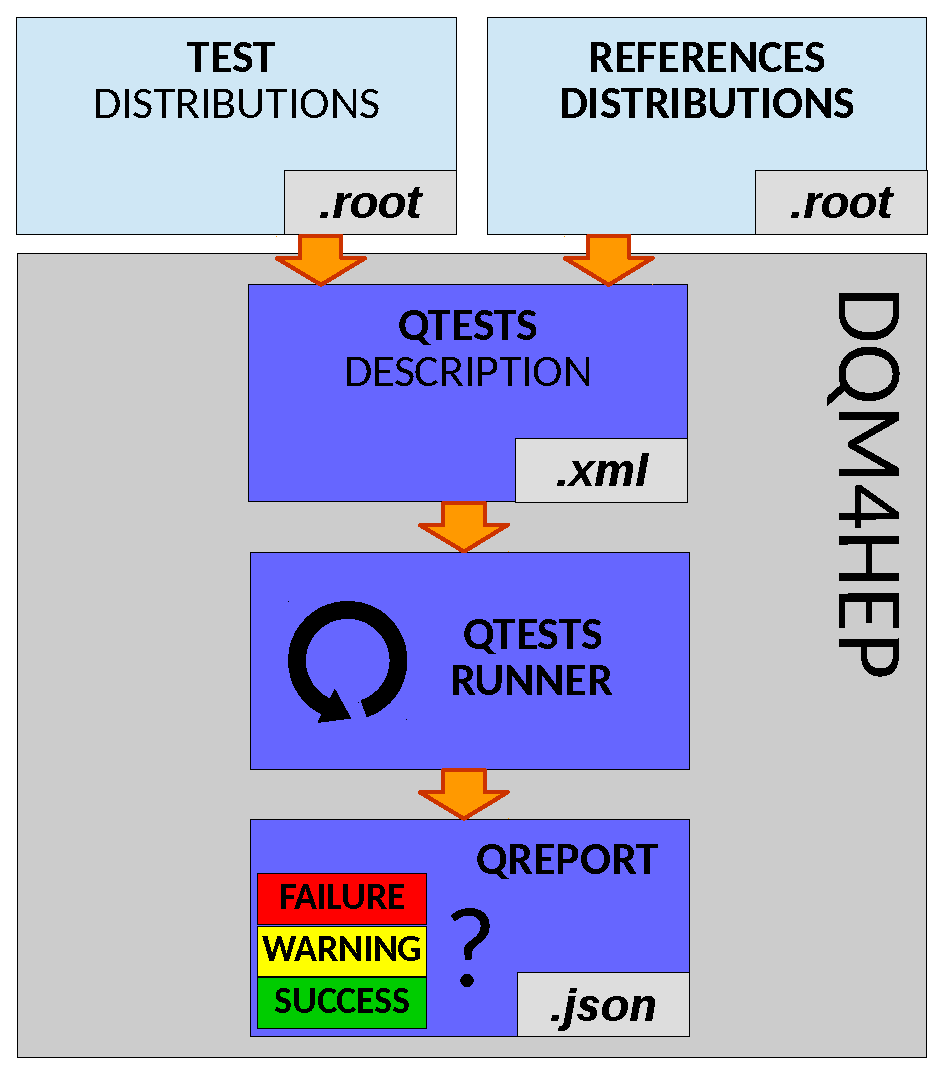
\includegraphics[width=0.95\linewidth]{figs/QTestRunner.pdf}      
    \end{center}
  \end{minipage}
  % \begin{center}
    \fcolorbox{black}{MyGray}{
    \tiny
    \begin{tabular}{lllll}
      \textbf{NAME}               &  \textbf{QTEST}    & \textbf{STATUS}  & \textbf{QUALITY}  & \textbf{MESSAGE} \\
      DblGaus\_Mean15\_RMS2\_RMS5 &  MeanAround15Short & \textcolor{MyGreen}{\bf SUCCESS} & 0.998484 & Expected 15, got 15.0019 \\
      Gaus\_Mean10\_RMS2          &  MeanAround10Long  & \textcolor{MyGreen}{\bf SUCCESS} & 0.997348 & Expected 10, got 10.0133 \\
      Gaus\_Mean10\_RMS2\_bck     &  MeanAround10Short & \textcolor{red}{\bf FAILURE}  & 0.388153 & Expected 10, got  5.6458
    \end{tabular}
    }    
  % \end{center}

\end{frame}


%----------------------------------------------------------------------
\begin{frame}
  \frametitle{The DQM4hep online architecture}
  \framesubtitle{DAQ data monitoring}
  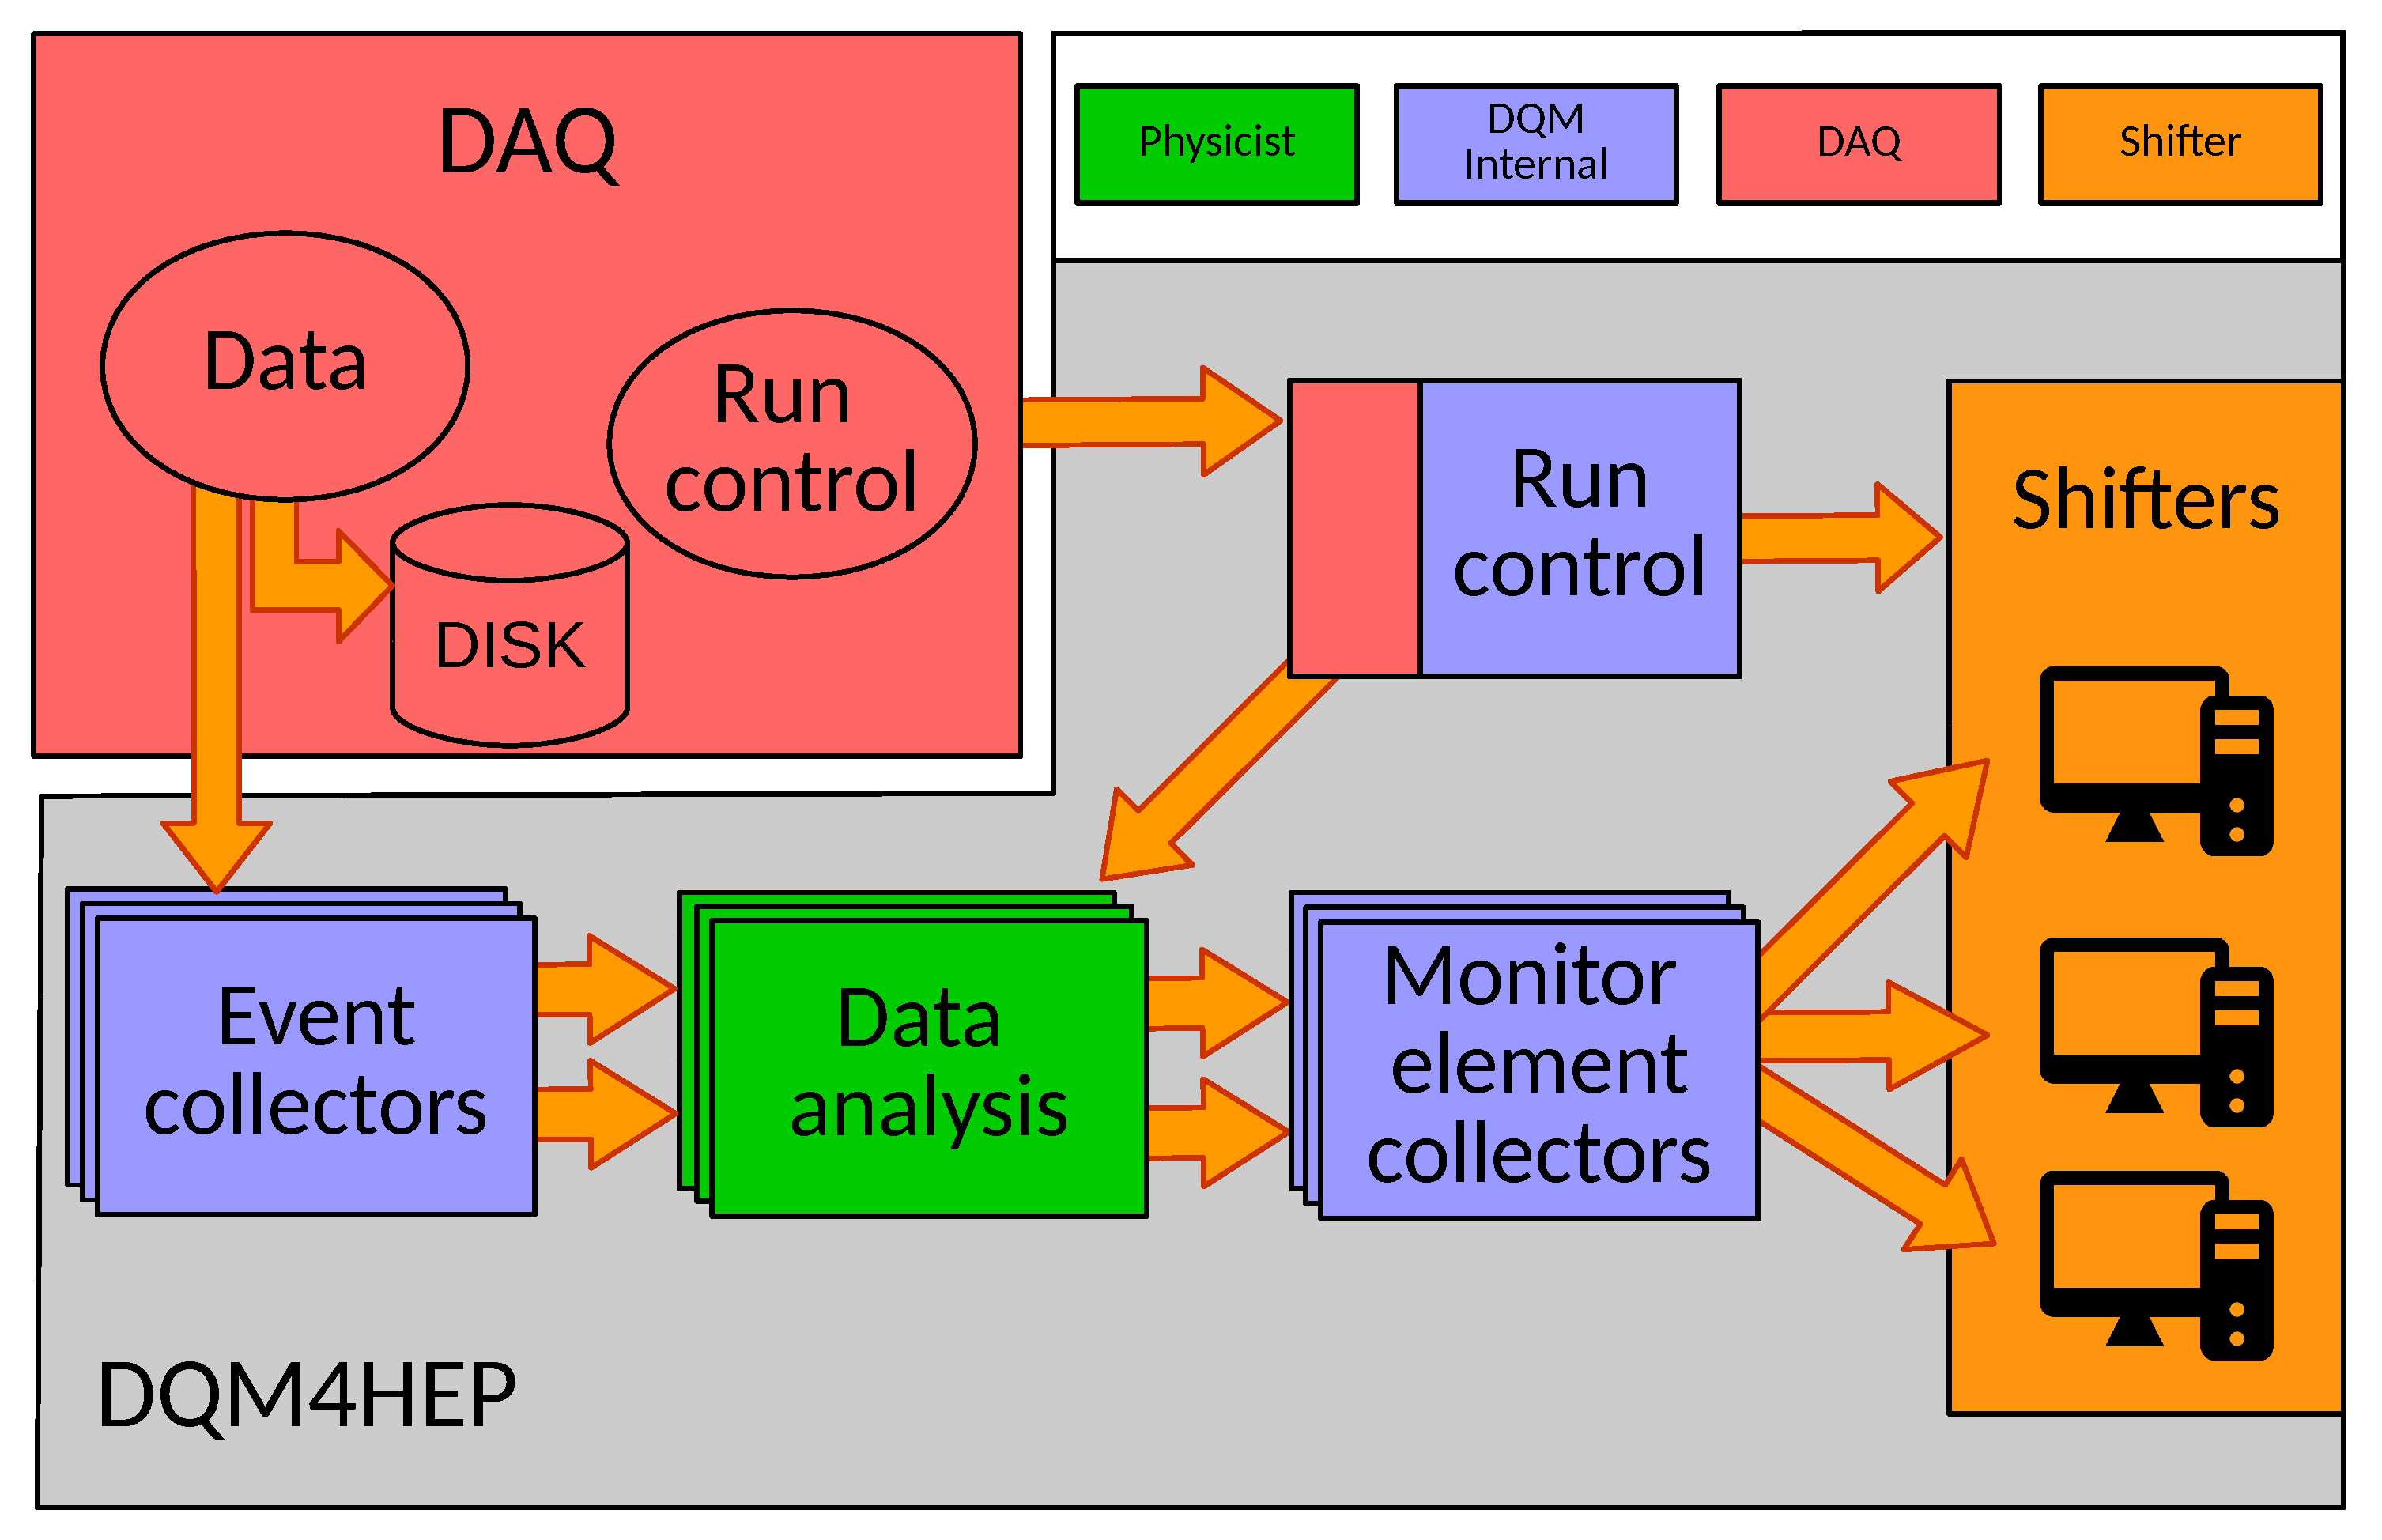
\includegraphics[width=0.95\linewidth]{figs/AnalysisModuleArchitecture.pdf}
\end{frame}

%----------------------------------------------------------------------
\begin{frame}
  \frametitle{The DQM4hep online architecture}
  \framesubtitle{Slow control data monitoring}
  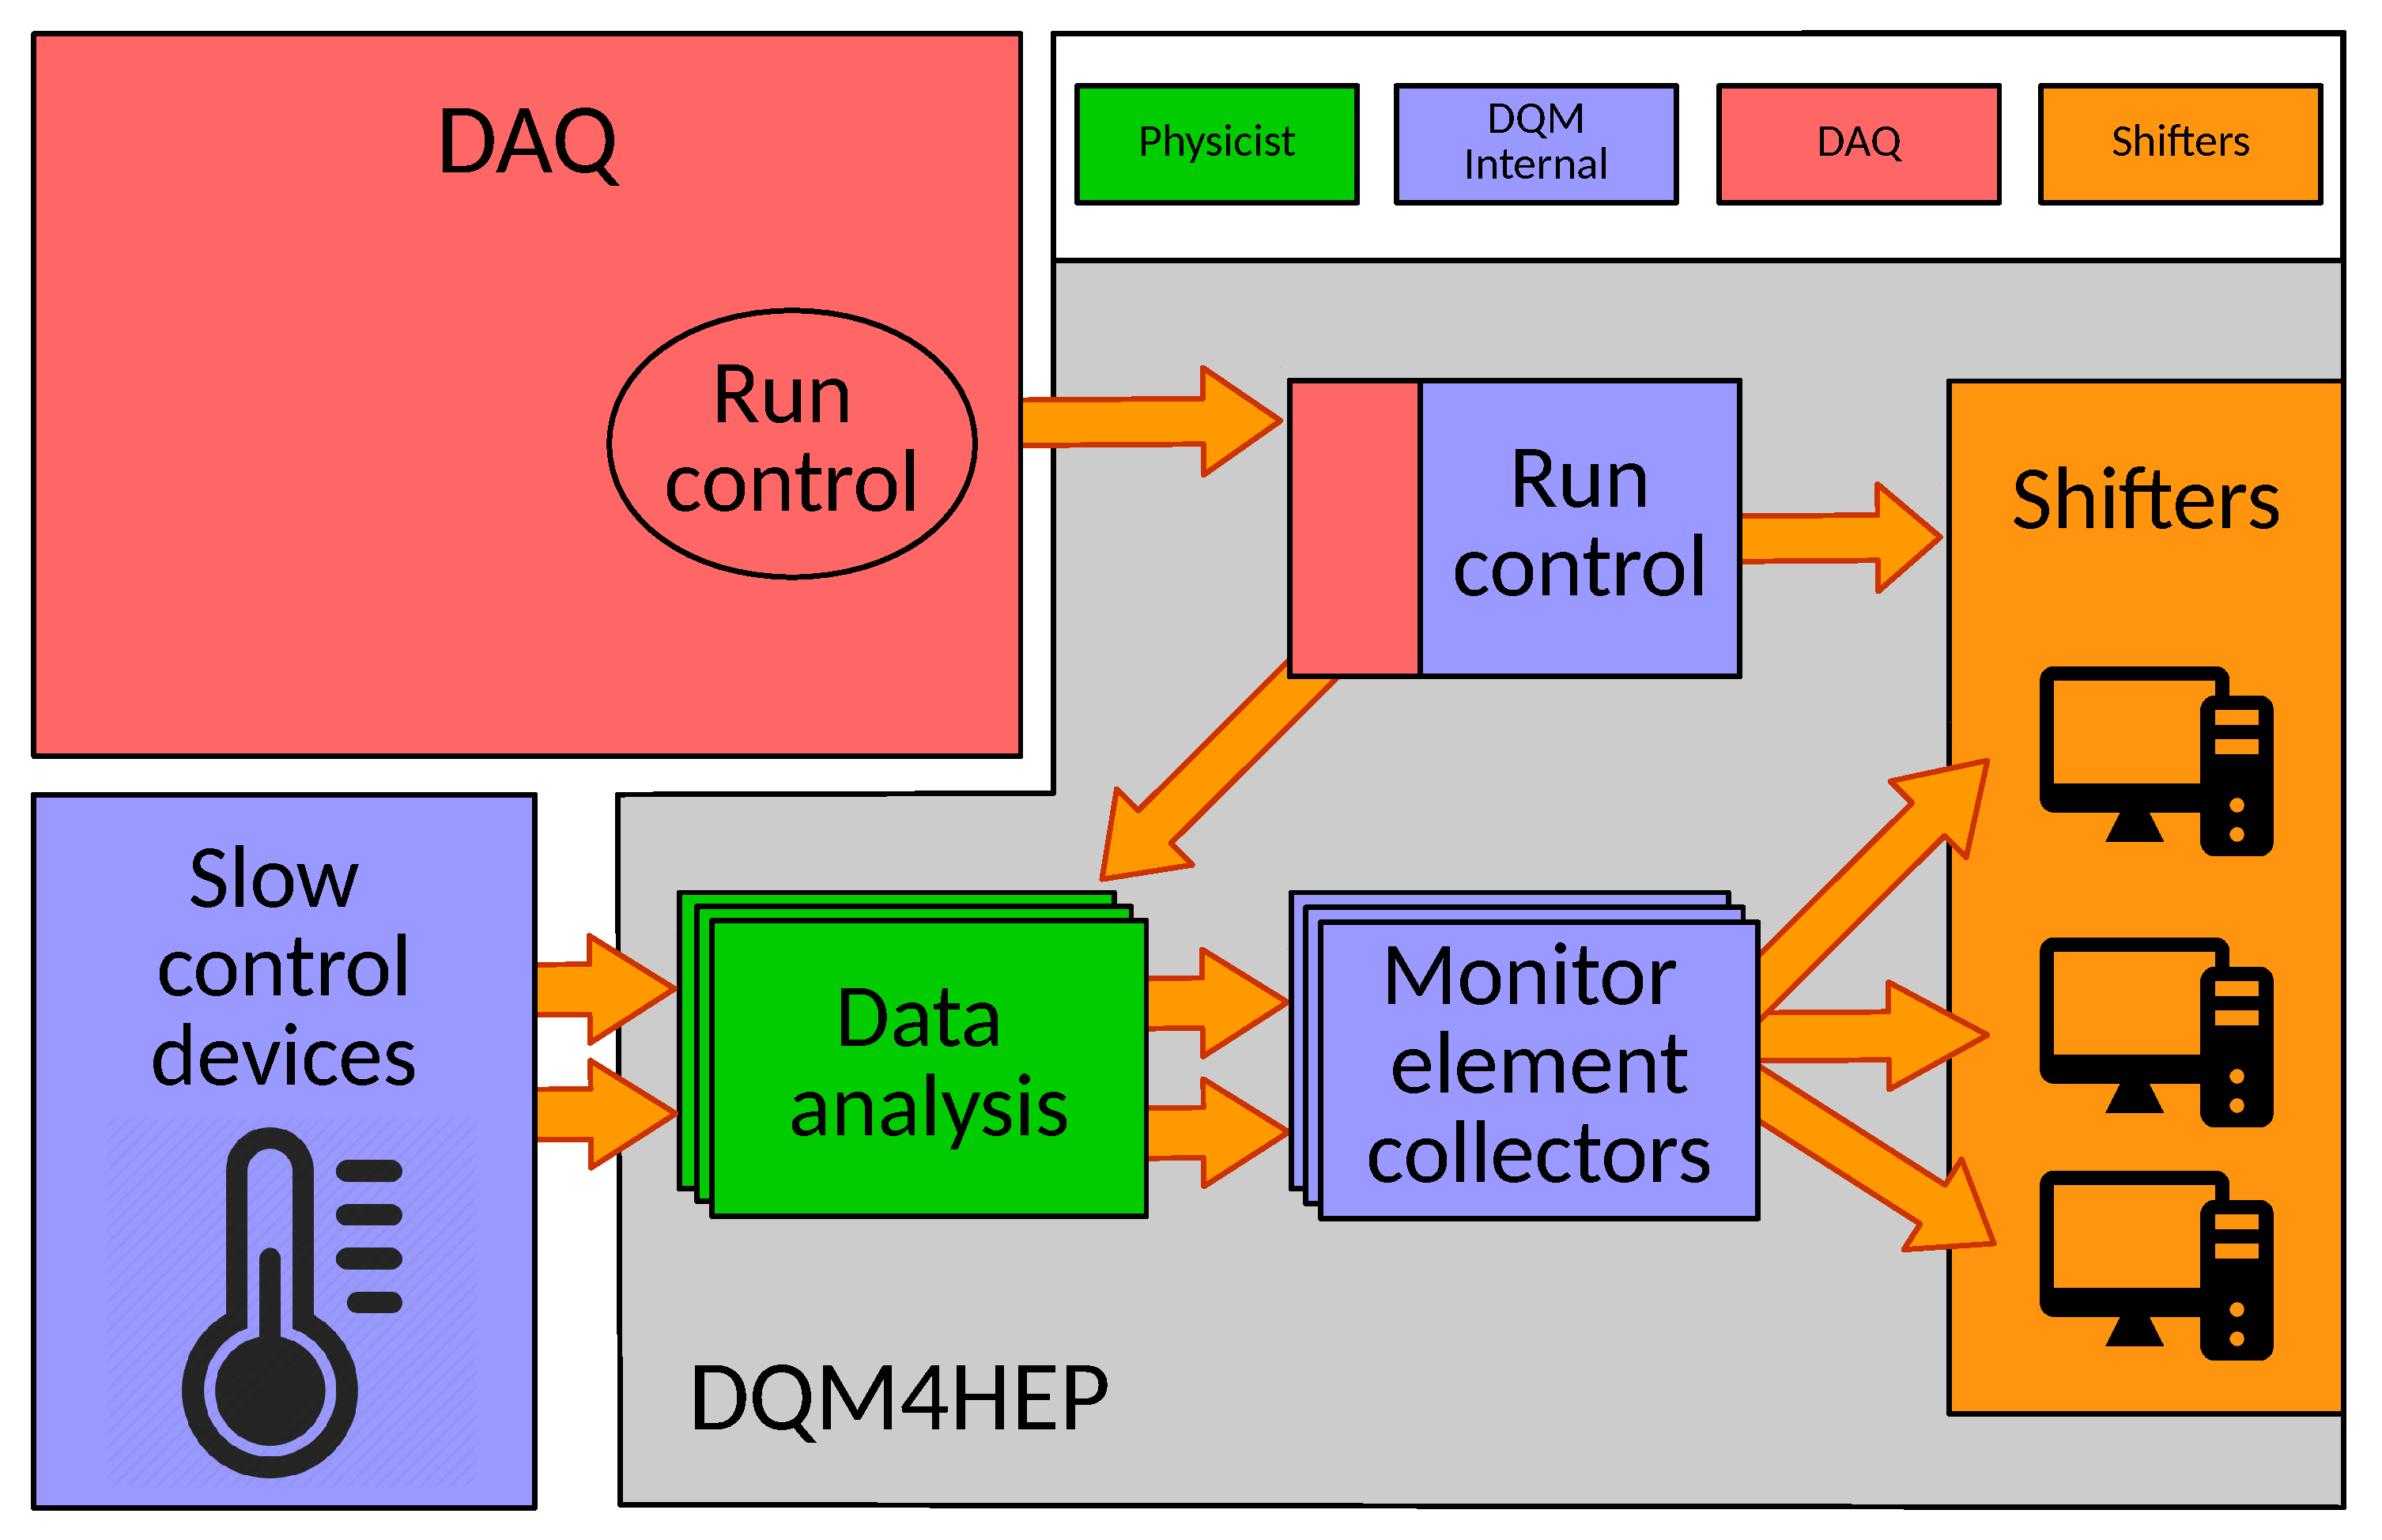
\includegraphics[width=0.95\linewidth]{figs/StandaloneModuleArchitecture.pdf}
\end{frame}

%----------------------------------------------------------------------
\begin{frame}
  \frametitle{The DQM4hep online architecture}
  \framesubtitle{Re-process DAQ data: file reader}
  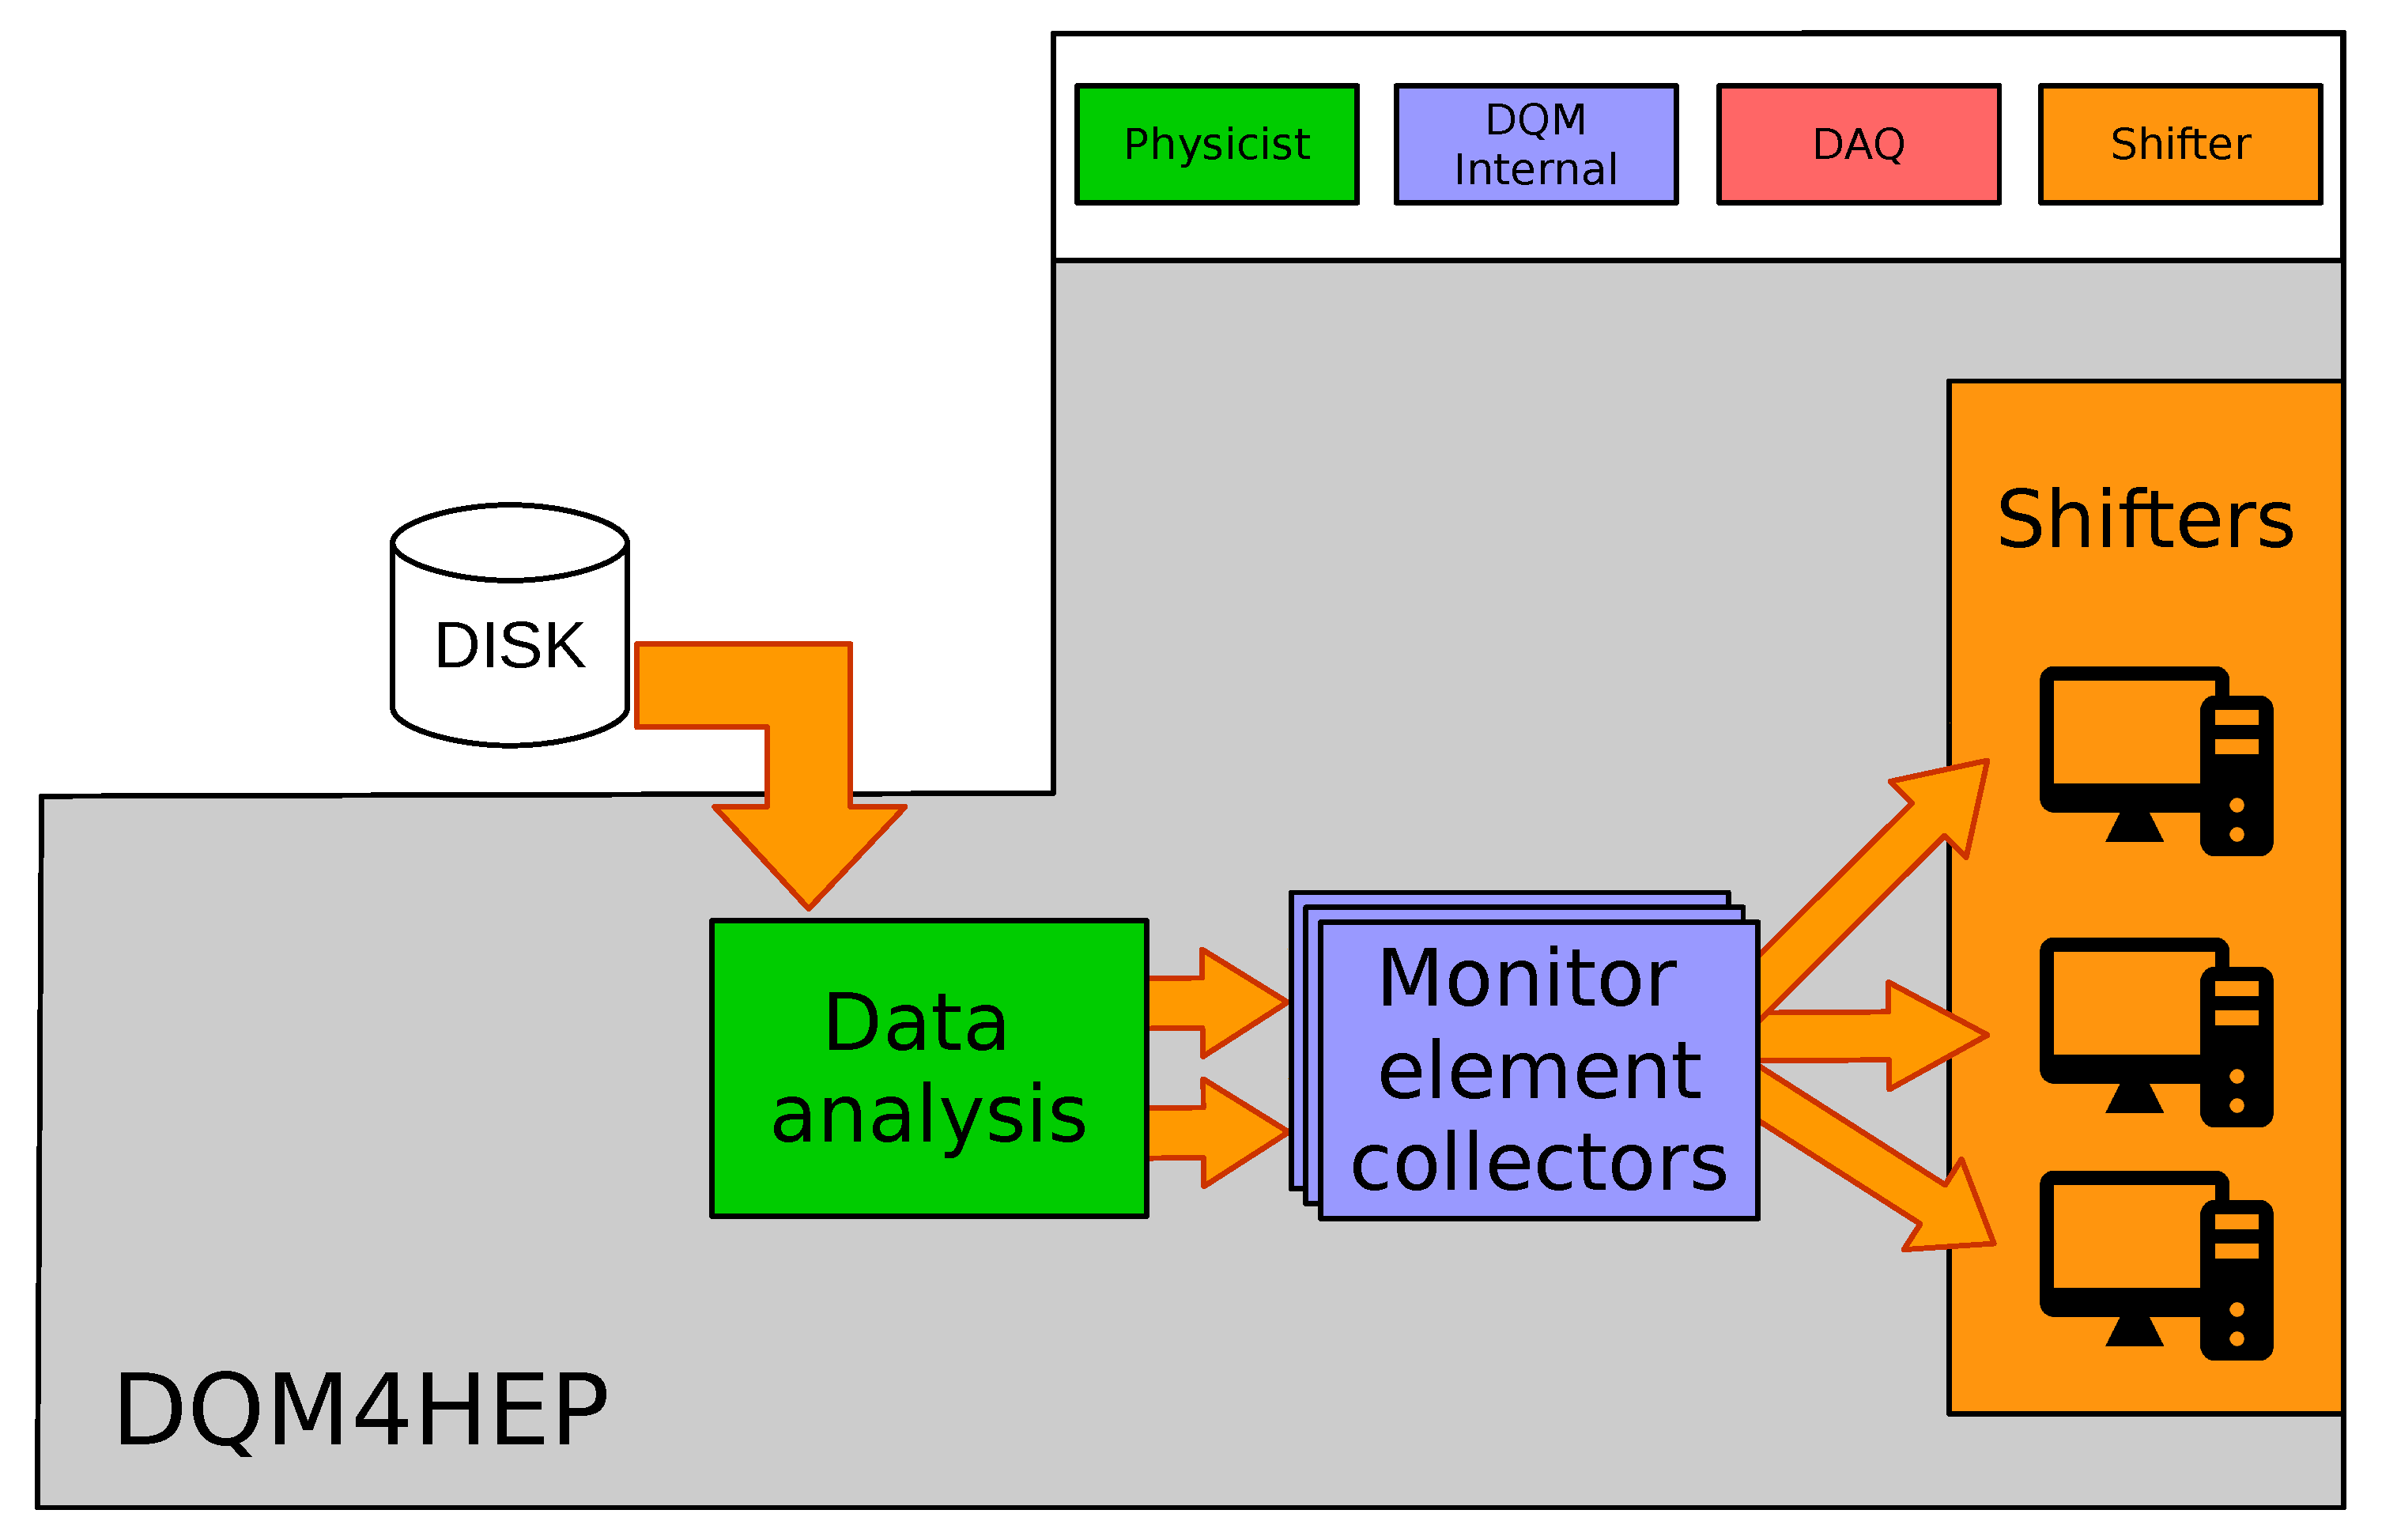
\includegraphics[width=0.95\linewidth]{figs/FileReaderModuleArchitecture.pdf}
\end{frame}

%----------------------------------------------------------------------
\begin{frame}
  \frametitle{Web monitoring interface. Ongoing ...}
  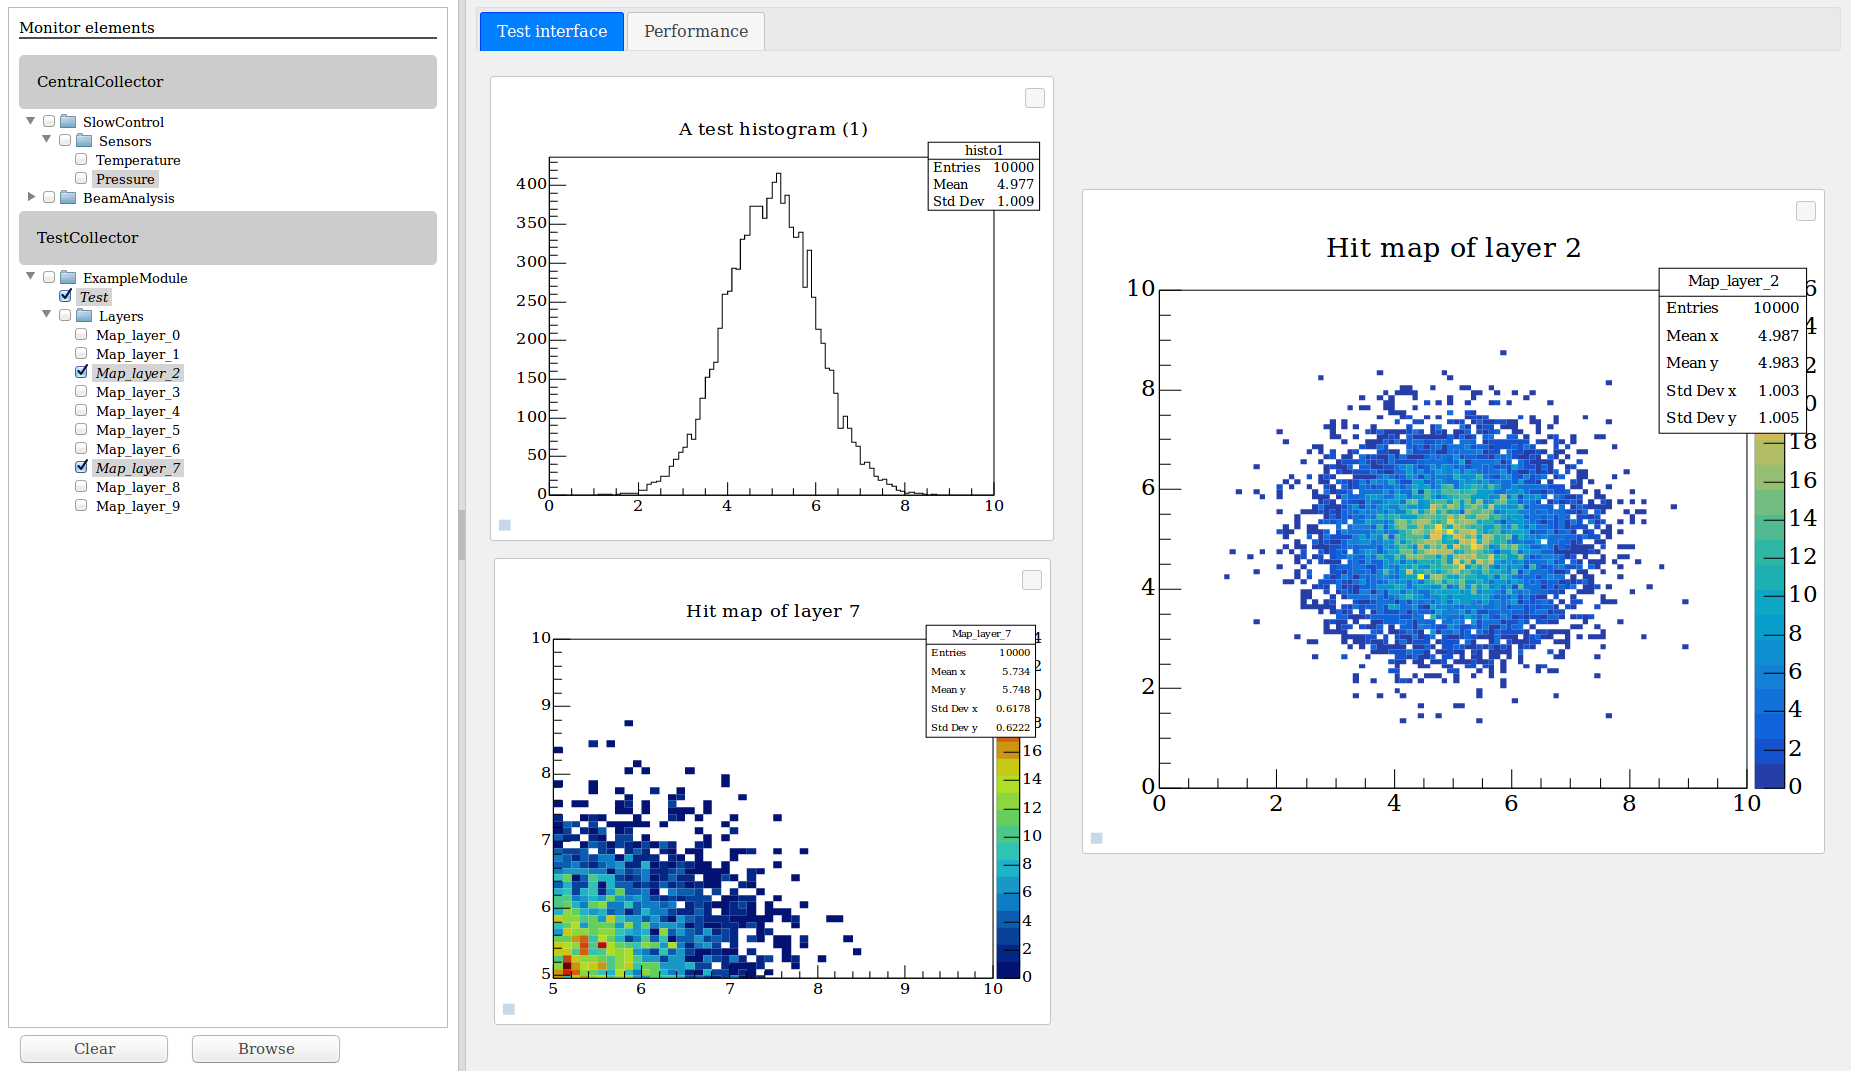
\includegraphics[width=\linewidth]{figs/ScreenshotWebMonitoring.png}
\end{frame}

%----------------------------------------------------------------------
\begin{frame}
  \frametitle{Web monitoring interface browser. Ongoing ...}
  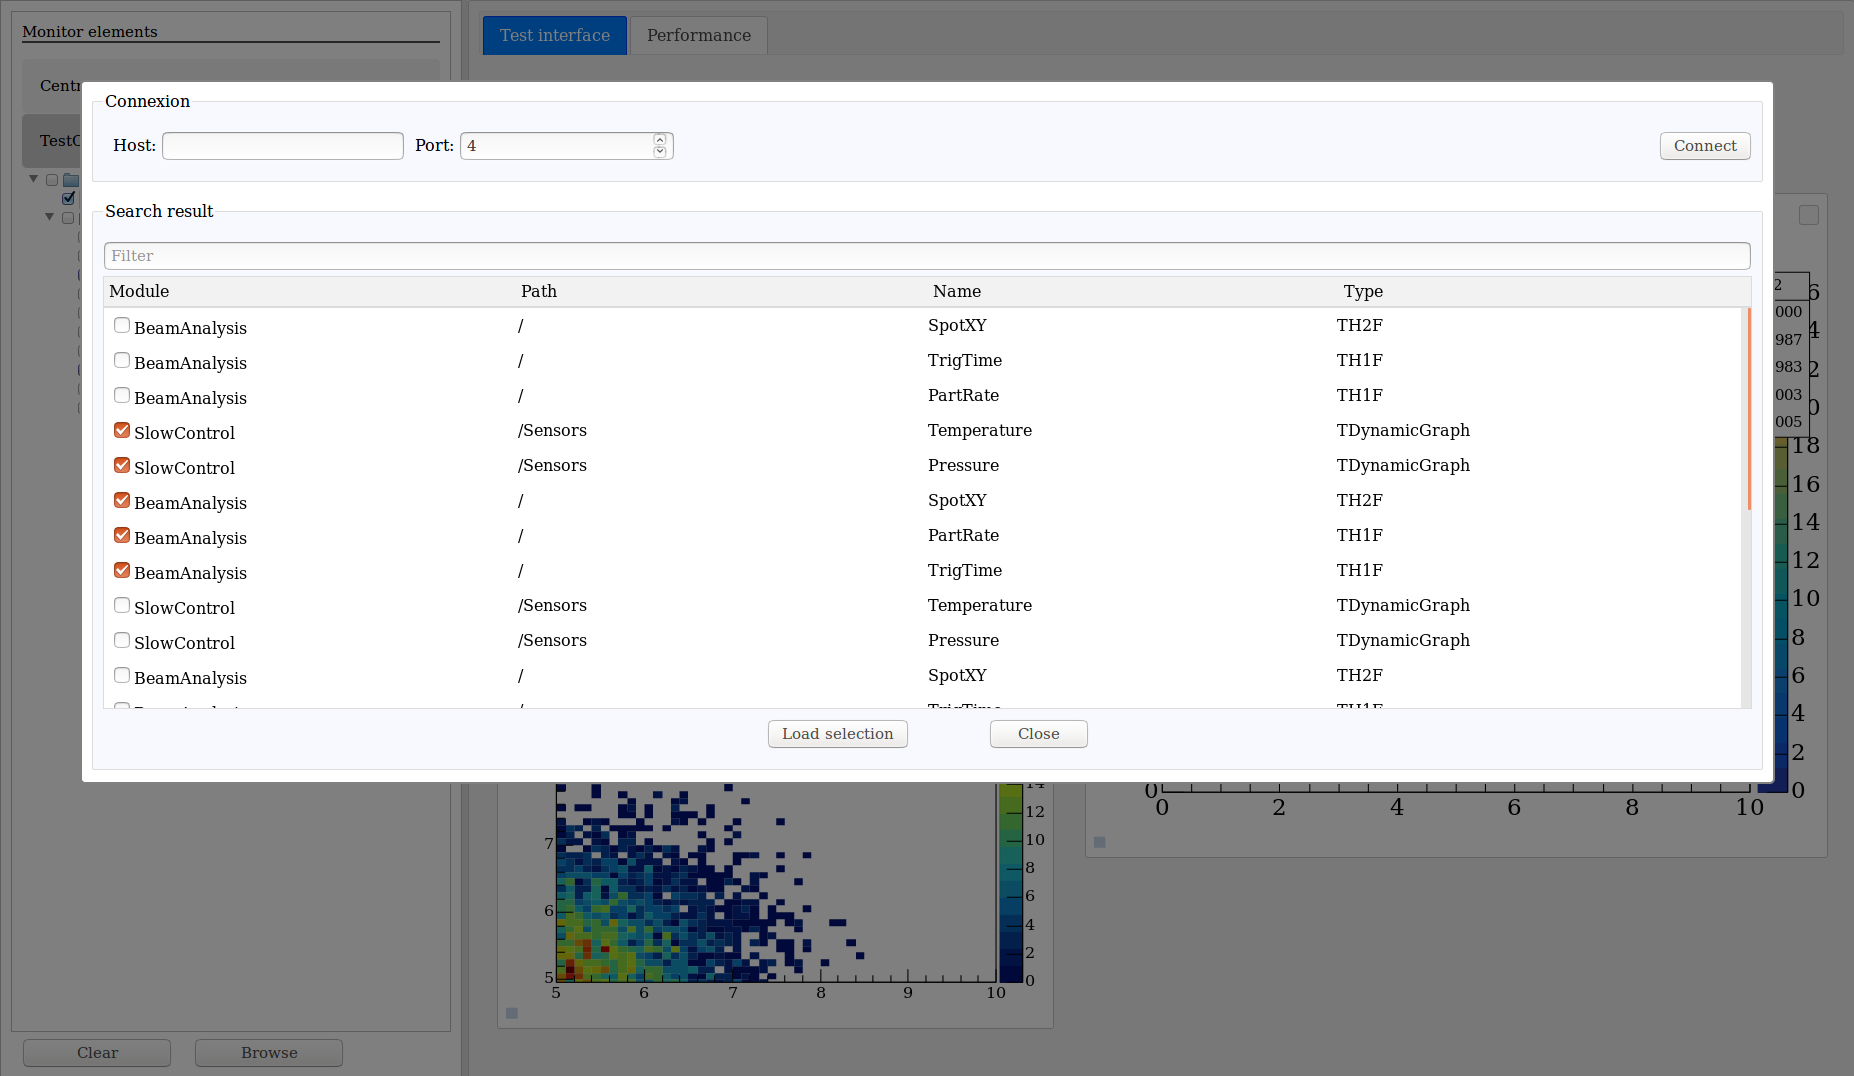
\includegraphics[width=\linewidth]{figs/ScreenshotWebMonitoringBrowser.png}
\end{frame}

%----------------------------------------------------------------------
\begin{frame}
  \frametitle{DQM4hep integration}
  % \footnotesize
  \begin{block}{Currently using DQM4hep}
    \begin{itemize}
      \item CALICE SDHCAL online system
      \begin{itemize}
        % \scriptsize
        \item Hit map, GRPC HV/current, beam analysis, electronics performances
      \end{itemize}
      \item CALICE AHCAL (quasi-)online system
      \begin{itemize}
        % \scriptsize
        \item Hit correlations, hit maps, SiPM currents, electronics performances
      \end{itemize}
    \end{itemize}    
  \end{block}
  \begin{block}{Future integration}
    \begin{itemize}
      \item EUDAQ framework (+ beam telescopes)
      \item ILCSoft simulation data monitoring (Continous integration)
      \item DREAM calorimeter (Dual-readout calorimeter)
      \item DAMIC experiment (Dark matter)
    \end{itemize}
  \end{block}
\end{frame}


%----------------------------------------------------------------------
\begin{frame}
  \frametitle{Ongoing work on software}
  \footnotesize
  Latest version is v01-04-04. Used as proof of principle. \\
  ~\\
  But, suffers from many things:
  \begin{itemize}
    \item Link to DAQ run control not possible. Run started manually...
    \item Clumsy ROOT Qt plugin installation. ROOT full installation often needed
    \item No separation between online and offline tools. All are online somehow...
  \end{itemize}
  ~\\
  New version coming soon !
  \begin{itemize}
    \item Moved to web visualization tools (js + JSROOT)
    \item Link to DAQ run control finally implemented
    \item Packages split into more granular sub-packages
    \begin{itemize}
      \scriptsize
      \item DQMCore, DQMNet, DQMOnline, DQMVisualization, etc...
    \end{itemize}
  \end{itemize}
  ~\\
  Next big steps:
  \begin{itemize}
    \item EUDAQ interface (AIDA2020)
    \item DESY slow control (AIDA2020) 
  \end{itemize}
\end{frame}


%----------------------------------------------------------------------
% \begin{frame}
%   \frametitle{DQM4hep software status}
%   \footnotesize
%   \textit{Most} of the features have been re-implemented from version v01-04-04.\\
%   ~ \\
%   \pause
%   \underline{Not yet finished}:\\
%   \begin{itemize}
%     \item Monitor element collector is re-implemented but not yet on master branch.
%     \item Visualization interface currently being ported from Qt-vis to Web (js)\\
%     $\rightarrow$ Non-obvious communication between C++ and javascript (ws)
%   \end{itemize}
%   ~\\
%   \pause
%   \underline{Not re-implemented}:\\
%   \begin{itemize}
%     \item Online system:
%     \begin{itemize}
%       \scriptsize
%       \item Process remote control
%       \begin{itemize}
%         \scriptsize
%         \item Process manager run on several hosts. Can fork processes on demand
%         \item Client interface to steer many process manager remotely
%       \end{itemize}
%       \item Old implementation highly insecure:\\
%       $\rightarrow$ anyone can start any process from anywhere ...
%     \end{itemize}
%     \item Visualization:
%     \begin{itemize}
%       \scriptsize
%       \item Application performance monitoring interface (memory, bandwidth, cpu, etc ...)
%       \item Run control interface. Legacy, will not be re-implemented ...
%       \item Remote process management client interface. Requires backend re-implementation
%     \end{itemize}
%   \end{itemize}
% \end{frame}

% %----------------------------------------------------------------------
% \begin{frame}
%   \frametitle{Web monitoring interface. Ongoing ...}
%   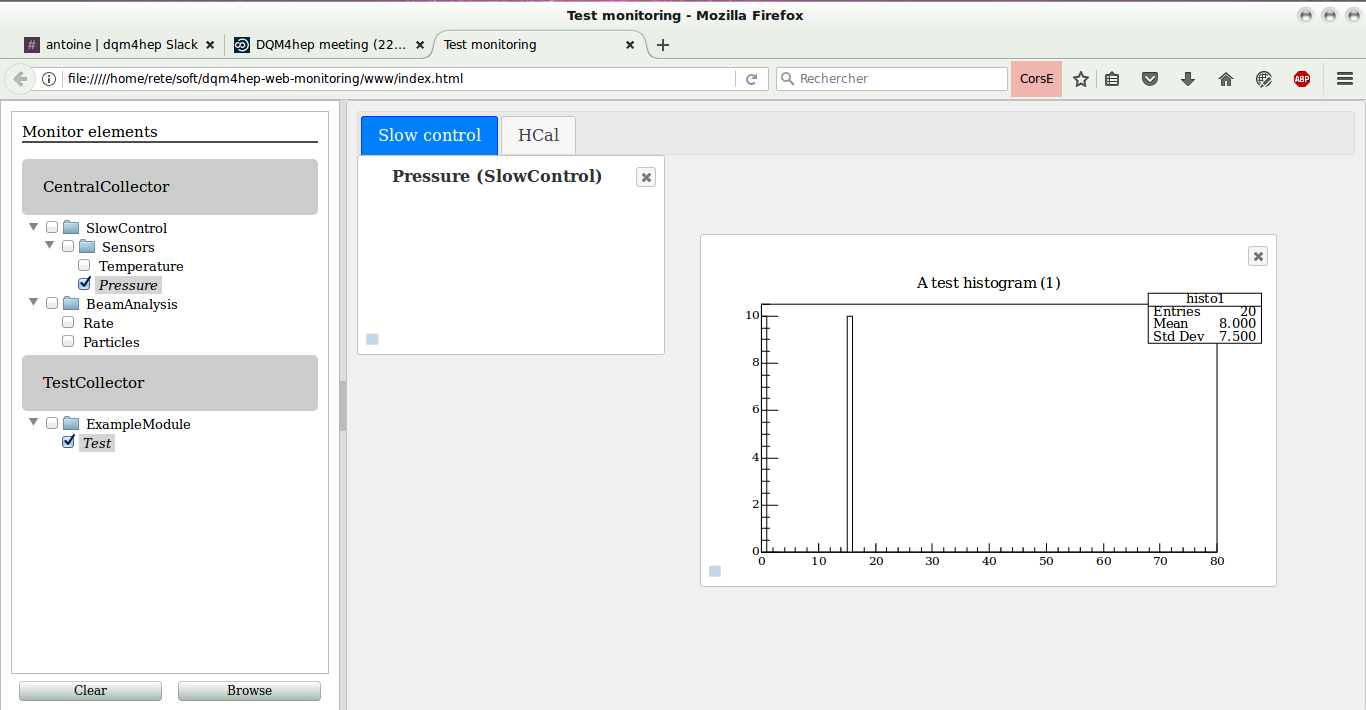
\includegraphics[width=\linewidth]{figs/DQMWebMonitoring-current-18-06-20.png} \\
%   ~ \\
%   Working on monitor element collector browser ...
% \end{frame}


% ----------------------------------------------------------------------
\begin{frame}
  \frametitle{Conclusion and outlook}
  Conclusion:
  \begin{itemize}
    \footnotesize
    \item A generic DQM software solution is being developed
    \item The abstract event interface allows different experiment to use it
    \item Prototypes/experiments already use it
    \begin{itemize}
      \scriptsize
      \item CALICE SDHCAL
      \item CALICE AHCAL
    \end{itemize}
    \item Currently finishing last master-piece: the web monitoring
  \end{itemize}
  ~ \\
  Outlook:
  \begin{itemize}
    \footnotesize
    \item Next major step is EUDAQ integration
    \begin{itemize}
      \scriptsize
      \item Will bring a full community as new users ! 
    \end{itemize}
    \item New integrations coming soon
    \begin{itemize}
      \scriptsize
      \item DAMIC experiment (Dark matter)
      \item DREAM Calorimeter
    \end{itemize}
    \item Allways looking for new collaborations !
  \end{itemize}
\end{frame}

%----------------------------------------------------------------------
\begin{frame}
  \frametitle{DQM4hep}
  \framesubtitle{URLs and contact}
  \footnotesize
  \underline{GitHub collaboration}\\
  \vspace*{0.1cm}
  ~~~
  \begin{minipage}{0.03\linewidth}
    
\includegraphics[width=\linewidth]{figs/github-logo.png}
  \end{minipage}
  \href{https://github.com/dqm4hep}{\tt https://github.com/dqm4hep} \\
  ~\\
  \underline{Documentation} \\
  \vspace*{0.1cm}
  ~~~
  \begin{minipage}{0.1\linewidth}
    
\includegraphics[width=\linewidth]{figs/doxygen-logo.png}
  \end{minipage}
  \href{https://dqm4hep.github.io/dqm4hep-doxygen/}{\tt https://dqm4hep.github.io/dqm4hep-doxygen/} \\
  ~\\
  ~~~
  \begin{minipage}{0.1\linewidth}
    
\includegraphics[width=\linewidth]{figs/readthedocs-logo.png}
  \end{minipage}
  \href{http://dqm4hep.readthedocs.io/en/latest/}{\tt http://dqm4hep.readthedocs.io/en/latest/} \\
  ~\\
  \underline{Slack channel} (Announcements, help, management) \\
  \vspace*{0.1cm}
  ~~~
  \begin{minipage}{0.035\linewidth}
    
\includegraphics[width=\linewidth]{figs/slack-logo.png}
  \end{minipage}
  \href{https://dqm4hep.slack.com}{\tt https://dqm4hep.slack.com} \\
  ~\\
  \underline{Citation} \\
  \vspace*{0.1cm}
  ~~~
  \begin{minipage}{0.05\linewidth}
    
\includegraphics[width=\linewidth]{figs/zenodo-logo.png}
  \end{minipage}
  \href{http://doi.org/10.5281/zenodo.1012575}{\tt http://doi.org/10.5281/zenodo.1012575} \\
  ~~~
  \begin{minipage}{0.05\linewidth}
    
\includegraphics[width=\linewidth]{figs/ieee-logo.png}
  \end{minipage}
  \href{https://doi.org/10.1109/NSSMIC.2016.8069668}{\tt 10.1109/NSSMIC.2016.8069668} \\  
  ~\\
  \underline{Contact us} !
  \begin{itemize}
    \scriptsize
    \item R. Ete (\href{mailto:remi.ete@desy.de}{\tt remi.ete@desy.de}) 
    \item A. Pingault (\href{mailto:antoine.pingault@ugent.be}{\tt antoine.pingault@ugent.be})
    \item T. Coates (\href{mailto:tc297@sussex.ac.uk}{\tt tc297@sussex.ac.uk})
  \end{itemize}
\end{frame}


%----------------------------------------------------------------------
\begin{frame}
  \frametitle{Backups}

\end{frame}


%----------------------------------------------------------------------
\begin{frame}
  \frametitle{The DQM4hep online system components}
  \footnotesize
  Provide monitoring of data recorded by the DAQ system. \\
  ~ \\
  Basic sub-components: \\
  \begin{itemize}
    \item \textbf{Run Control}\\
    $\rightarrow$ DQM application receiving commands/state/config from DAQ run control.\\
    $\rightarrow$ Forward it to DQM applications
    \item \textbf{Run Control Interface}\\
    $\rightarrow$ Interface to connect to DAQ run control, used by the DQM run control
    \item \textbf{Event Streamer}\\
    $\rightarrow$ Convert DAQ event structure $\leftrightarrow$ binary
    \item \textbf{Event Source}\\
    $\rightarrow$ DQM component to be integrated into DAQ to send events to DQM
    \item \textbf{Event Collector}\\
    $\rightarrow$ Collect events from event sources and re-distribute to DQM applications
    \item \textbf{Module}\\
    $\rightarrow$ Analyse data from DAQ or other data source (e.g slow control). \\
    $\rightarrow$ Produces monitor elements and run quality tests
    \item \textbf{Monitor Element Collector}\\
    $\rightarrow$ Collect monitor elements from modules and re-distribute them to shifters
  \end{itemize}

\end{frame}

%----------------------------------------------------------------------
\begin{frame}
  \frametitle{Old Qt4 GUI monitoring interface}
  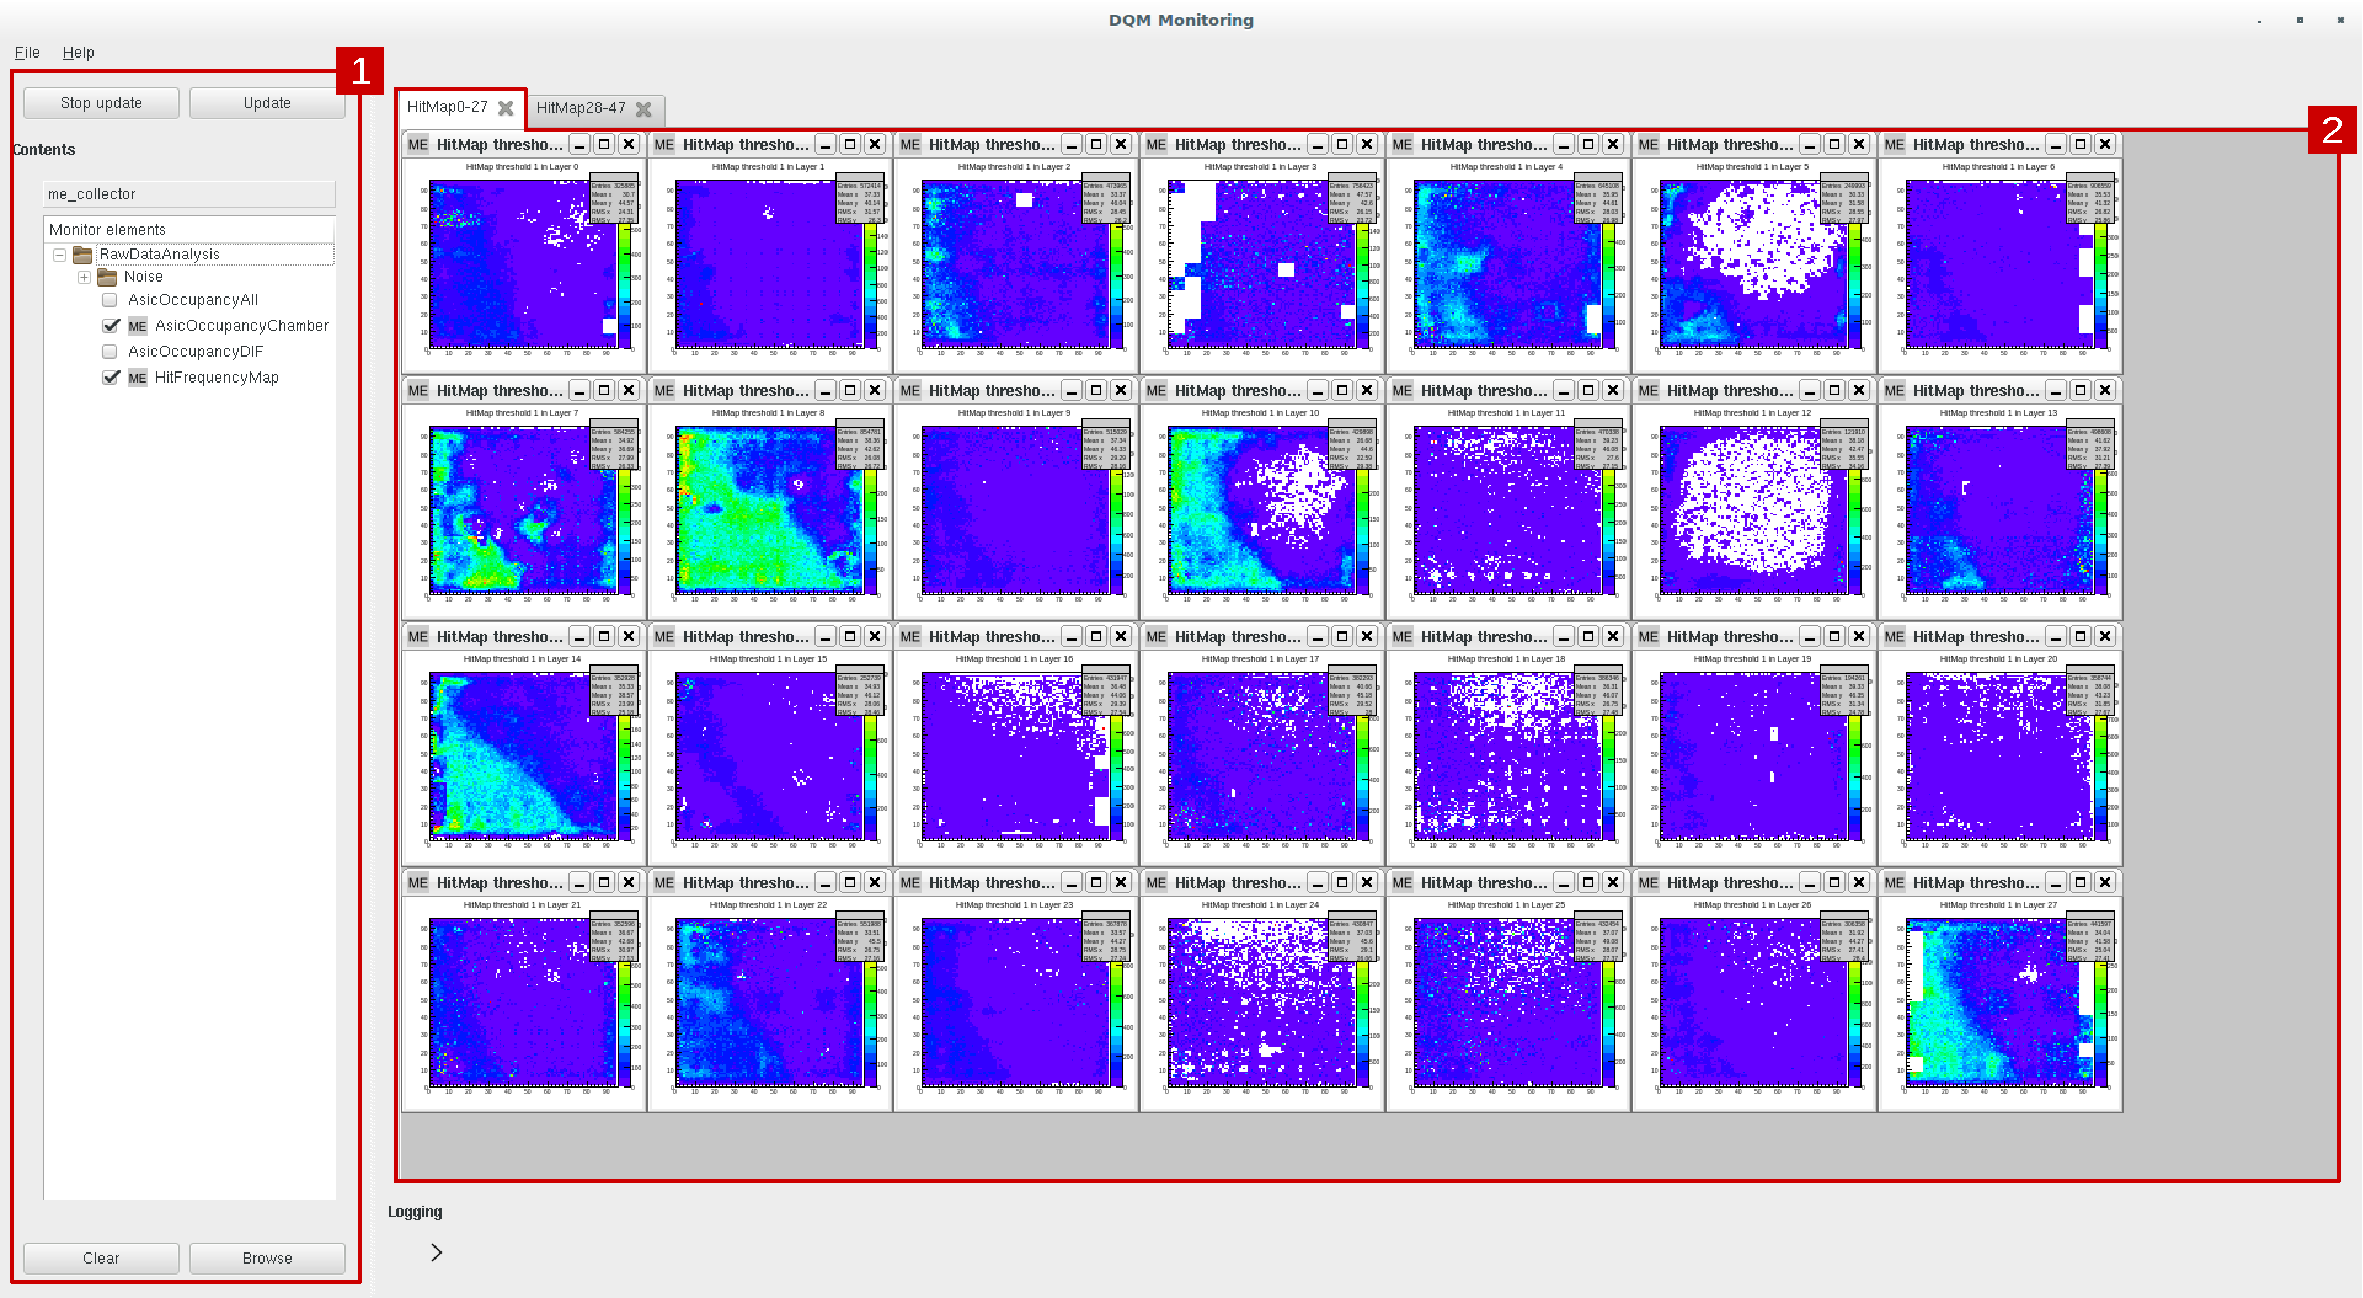
\includegraphics[width=\linewidth]{figs/MonitoringMainWindowGui.pdf}
\end{frame}

%----------------------------------------------------------------------
\begin{frame}
  \frametitle{Old Qt4 GUI monitoring browser}
  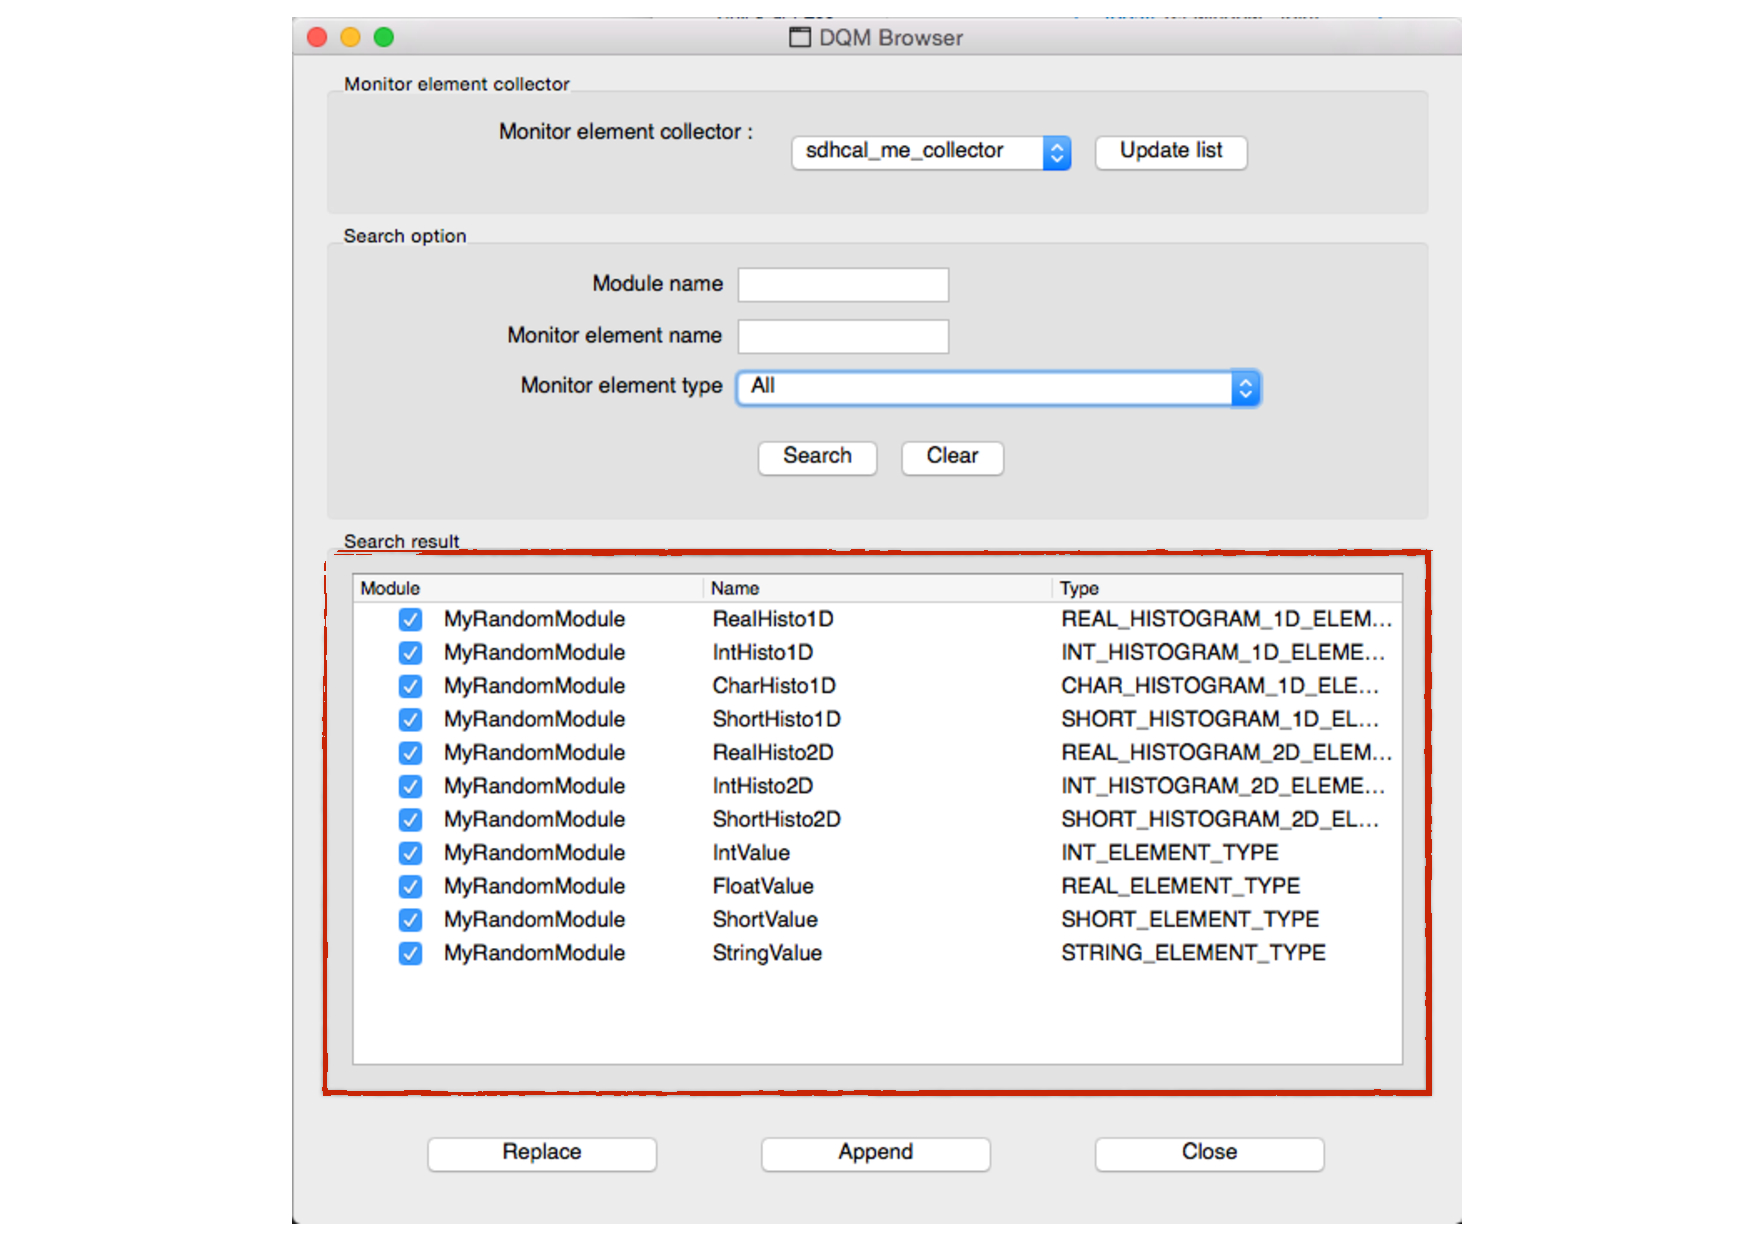
\includegraphics[width=\linewidth]{figs/Browser_SearchResultsAll.pdf}
\end{frame}

\end{document}



% Enable spell checker for vim
% setlocal spell spelllang=en
